\subsection{Bound-state with filled Fermi-sea\label{subsec:oneMolInFermiSea}}
Let us look into a bound level with the Fermi-sea background.  It  is the many-body effects from open-channel to close-channel although a more realistic model is to have two-channel solved self-consistently.  For a bound wave-function $\chi_{\vk_1,\vk_2}$, we have equation 
\begin{equation}
\hm\br{k_1^2+k_2^2}\chi_{\vk_1\vk_2}+\int{}d\vp{}v\br{p}\chi_{\vk_1-\vp,\vk_2+\vp}=E\chi_{\vk_1,\vk_2}
\end{equation}
Here the interaction $v\br{p}$ is only about the relative coordinator between two particles.  If we only consider only the central momentum 0 solution, $\vk_1=-\vk_2=-\vk$, the above equation can be reduced to 1-particle equation
\begin{equation}\label{eq:kSch}
\hm\br{2k^2}\chi_{\vk}+\int{}d\vp{}v\br{p}\chi_{\vk+\vp}=E\chi_{\vk}
\end{equation}
Now let us apply the restriction that Fermi sea is filled and not available.  $\chi=\overline{\chi^0}+\delta\chi$, where $\chi^0$ is the solution to the above equation \eqref{eq:kSch} in free space without the filled Fermi sea.  And $\overline{\chi^0}$ is simply the same wave-function removed all the component below Fermi level. 
\begin{equation}
\overline{\chi^0_\vk}=\begin{cases}0&k<k_F\\\chi^0_\vk&k\geq{}k_F\end{cases}
\end{equation}
And eq \eqref{eq:kSch} becomes 
\begin{equation}\label{eq:chiPerturb}
2\epsilon_k\delta\chi_\vk-\int\limits_{\abs{\vk+\vp}<k_F}d\vp{}v(p)\chi^0_{\vp+\vk}+\int\limits_{\abs{\vk+\vp}>k_F}d\vp{}v(p)\delta\chi_{\vp+\vk}=E\delta\chi_\vk+(E-E^0)\overline\chi^0
\end{equation}
%\textbf{Note: this is only correct if $E$ does not change. Otherwise, there is a term of $\delta{E}\overline\chi^0$} 

\begin{figure}[hbt]
\centering
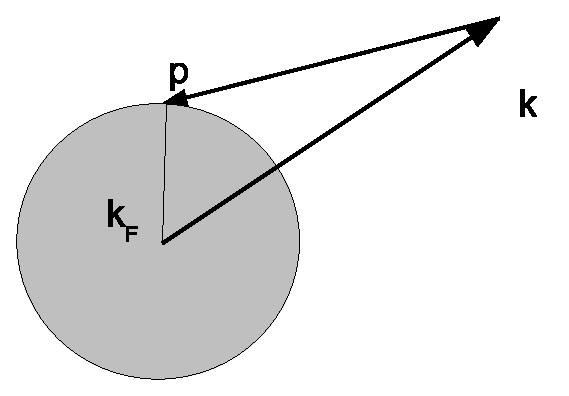
\includegraphics[width=.30\textwidth]{image/k+pVec.eps}
\caption{$\vk+\vp$}
\label{fig:k+pVec}
\end{figure}
Here $\chi^0(\vk)$'s extension is much smaller than $1/a_0$, in that region, $v(p)\approx{}v\br{p=0}=v_0$ because it is short-range potential within $a_0$.  
\[
\int\limits_{\abs{\vk+\vp}<k_F}d\vp{}v(p)\chi^0_{\vp+\vk}=v_0\int\limits_{\abs{\vk'}<k_F}d\vk'{}\chi^0_{\vk'}=v_0\chi^0_{\vk=0}\frac{4\pi}{3}k_F^3=\nth{2}v_0\chi^0_{\vk=0}n\equiv{}A(n)
\]
the second equation uses the fact that, as $\chi^0(r)$'s extension is much smaller than $1/k_F$, in the region $\abs{\vk'}<k_F$, $\chi^0_{\vk'}\approx\chi^0_{\vk'=0}$.  And $\frac{4}{3}\pi{}k_F^3=\nth{2}n$, where $n$ is the density of the fermions. So the eq \eqref{eq:chiPerturb} can be further simplified into, \emph{provided the last term can be ignored (NOT GOOD APPROX)} 
\[
2\epsilon_k\delta\chi_\vk-A(n)+v(p=0)\int\limits_{\abs{\vk}>k_F}d\vk{}\delta\chi_{\vk}=E\delta\chi_\vk
\]
And we have 
\begin{equation}\label{eq:deltaChi}
\delta\chi_\vk=\frac{A(n)-v_0\int_{\abs{\vk}>k_F}d\vk{}\delta\chi_{\vk}}{-E+2\epsilon_k}
\end{equation}
We noticed that the nominator is a constant.  The first term is negative, while the second is positive.  Also $E=-\hbar^2/{2ma_c^2}<0$, and $a_0\ll{}a_c\ll{}1/{k_F}$, in the region where we are most interested, $\abs{E}\sim\epsilon_k$.  This is very much like the $F_k$ in the BCS, and its Fourier transformation is a bound-state fall off at the scale of $a_c$ as in $E$. So it is more like just the normalization of the close-channel bound state are modified without the wave-function changes. 

This whole approach is like Cooper problem, which misses the pair interaction.  Is that all we miss here? Possible improvement:
\begin{itemize}
 	\item To solve two-channel self-consistently instead fixing open-channel to occupy all the Fermi-sea. It seems to be the most relevant to the narrow-resonance.
 	\item To introduce interaction of the close-channel bound state.  Unlikely, it is still realative small comparing to $1/k_F$ and they probably do not interact much. But there are two aspects:  relative coordinate and the central of mass.  Relative coordinate may not change, but central of mass can go through something like BEC.  Or maybe not? 
 	   
 \end{itemize} 
To find the new $E$, we need to integrate the RHS of eq \eqref{eq:deltaChi}, and this diverges in high $k$ over $k>k_F$.  It needs either some cutoff or renomalization.  

In terms of the eq \eqref{eq:chiPerturb}, should we put in one more term $(E-E^0)\overline{\chi^0}$ on the RHS? 
\subsection{Tony's comment}
He kind of like the approach.  He suggest me to solve eq \eqref{eq:deltaChi} by integration with a cut off.  The divergence comes from $v(p=0)$ and that should gives a pausible cutoff.  
